%!TEX root = ../thesis.tex
%Adding the above line, with the name of your base .tex file (in this case "thesis.tex") will allow you to compile the whole thesis even when working inside one of the chapter tex files
\chapter{Coronal Mass Ejection and Plasma Shock Theory} 
\label{chap:2}

\section{Plasma Physics and Magnetohydrodynamics}\label{sec:1}

\subsection{Maxwell's Equations}\label{sec:10}

\begin{eqnarray}
\nabla \cdot E &=& \frac{\rho}{\epsilon_0} \\
\nabla \cdot B &=& 0 \\
\curl{E} &=& - \frac{dB}{dt} \\
\curl{B} &=& \mu_0 j + \frac{1}{c^2}\frac{dE}{dt} 
\end{eqnarray}



\subsection{Plasma Physics and Boltzmann Equation}\label{sec:11}

\subsection{Magnetohydrodynamics}\label{sec:12}

\subsection{Magnetic Reconnection}\label{sec:13}

\subsection{MHD Rankine-Hugoniot Equations}\label{sec:14}

\subsection{Bow Shocks}\label{sec:15}



\section{Coronal Mass Ejections}\label{sec:2}

\subsection{Catastrophe Model}\label{sec:20}

\subsection{Magnetic Breakout Model}\label{sec:21}

The magnetic breakout model was first proposed by \citep{antiochos1999} and involves a quadrupolar (or more complex) magnetic flux system. A core magnetic field is flanked by two side-lobe fields, which collectively lie underneath an over-arching field that stabilizes the whole system. The overarching field and core field are almost anti-parallel, creating a magnetic null point between the two Figure~\ref{fig:breakout_model}. Non potentiality is injected into the core by twisting/shearing of the foot points or by flux emergence. This non-potentiality causes the core field to grow and encounter the overarching field, distorting the null point into a current sheet and eventually allowing reconnection to occur. The reconnection removes field lines from the overarching field and adds it to the side-lobe systems, allowing further growth of the core field. The growth of the core field in turn drives further breakout reconnection resulting in a positive feedback required for explosive expulsion of the core. Finally, as the core is accelerated a current sheet forms in its wake, eventually leading to a separation of the core flux from the solar surface that forms a plasmoid structure typical of a three part CME \citep{lynch2004}; an important aspect of this is that flux rope formation happens as a consequence of eruption i.e., it is not pre-existing. The magnetic breakout model was used to circumvent the Aly-Sturrock limit \citep{aly1991, sturrock1991} i.e., it allowed a flux system to erupt, without having to open the constraining field lines to infinity.
\begin{figure}[!b]
\begin{center}
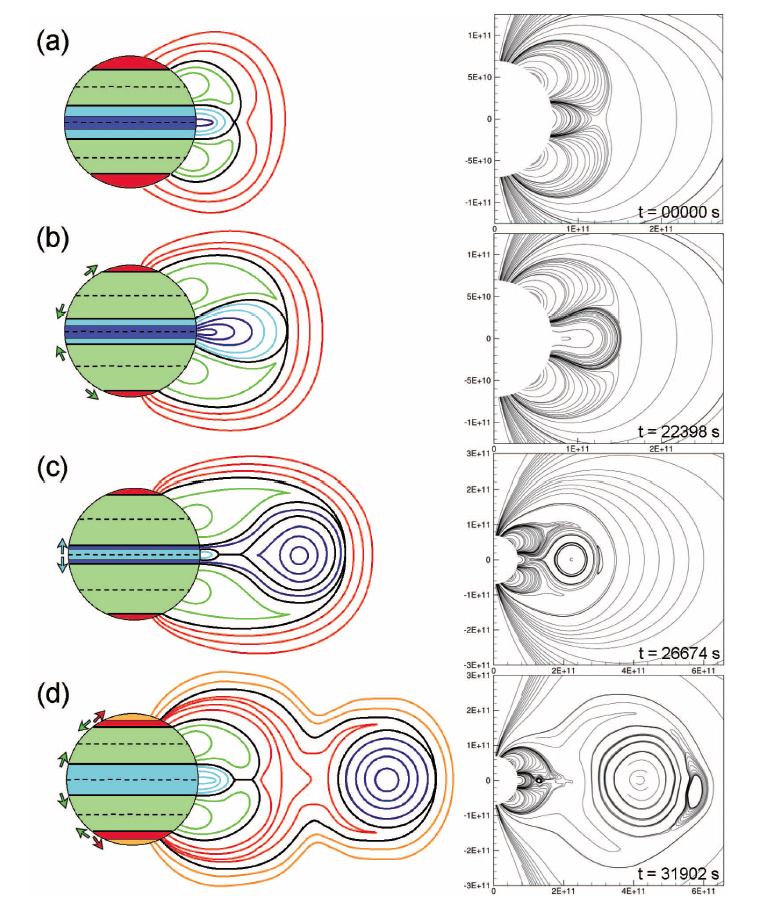
\includegraphics[scale=0.55]{images/lynch_breakout}
\caption{The breakout model, consisting of a quadrupolar flux system in which the central flux (blue) is flanked by to side lobe flux systems (green), with the entire system kept in stability by the tension of the overlying red field. Shearing and/or twisting on the underlying flux causes it to grow slowly. Eventually a current sheet forms at the magnetic null above the central flux, causing reconnection. This reconnection transfers overlying field to the side-lobes, effectively creating a conduit for the central flux to escape as a CME \citep{lynch2008}.}
\label{fig:breakout_model}
\end{center}
\end{figure}
\clearpage
Kinematically, the CME/central field system should experience a slow rise (1\,km\,s$^{-1}$) for several hours due to shearing/twisting of the foot points. Once breakout reconnection has begun the CME experiences a much larger acceleration (100\,km\,s$^{-1}$). The reconnection in the current sheet in the wake of the CME is the source of energetic particles that ultimately lead to flaring (ribbons and soft x-ray loops). Therefore magnetic breakout predicts that the flaring process and SXR peak should only begin after CME acceleration (after breakout reconnection) has begun \citep{lynch2004}. However, the precedence in breakout reconnection over flaring reconnection may not always be case, with the latter sometimes driving the former \citep{macneice2004}. 

There has been observational tests of the magnetic-breakout model, showing it to be a viable explanation of some flaring and CME events, the most notable of which is the Bastille Day event \citep{aulan2000}. The observational signatures of the model include the presence of a null point in the corona above a complex multipolar flux system (inferred from potential field source surface extrapolations), a radio source imaged to be above the erupting structure (implying a reconnection site), and radio bursts beginning at frequencies indicative of high altitude (again indicating energy release above the erupting structure, prior to eruption) \citep{mano2003}. However, in some instances magnetic breakout is implied by observations of the above, but the kinematics are inconsistent with model predictions. For example the model predicts a long slow rise of the central flux system as the underlying field is increasingly sheared, after which there is a rapid acceleration once breakout reconnection is initiated. However, in the study of \citet{bong2006} the breakout reconnection occurred at the end of the CME acceleration phase, prompting a two-phase acceleration scenario.


\subsection{Toroidal Instability}\label{sec:22}

The toroidal instability model incorporates a pre-existing flux rope structure that is built from a torus of magnetic flux, some of which is buried beneath the photosphere \citep{chen1989}. The flux system is can be broken down into a combination of toroidal magnetic, toroidal current and a poloidal magnetic field and current Figure~\ref{fig:chen_model}. This flux rope system is embedded in a surrounding coronal magnetic field $B_{corona}$. The stability of the system depends on the nature of the $J \times B$ force due to the interaction toroidal and poloidal components of both the field and current. The interaction of $J$ and $B$ internal to the flux rope is usually termed the Lorentz self-force or the \textquoteleft hoop' force. An instability may be induced via twisting of the fluxrope footpoints to increases the amount of poloidal flux (effectively increasing the helicity of the system). Once the instability is induced, the fluxrope begins a bulk motion as well as a growth in its semi-minor axis. Hence the motion of the system can be analysed by looking at the central axis or the minor axes (leading and trailing edges. The three axes display slightly different kinematics e.g., the leading edge has a faster velocity than the trailing edge (due to fluxrope expansion). this has proved a useful test of the model when comparing the observations of erupting fluxrope structures as seen in white-light coronagraphs. \citet{krall2001} looked at the leading a trailing edges of erupting flux ropes, as well as the rope aspect ratio, an compared the observations to model expectations. Good agreement is found between the model kinematics and aspect ratio and the observed events.
\begin{figure}[!t]
\begin{center}
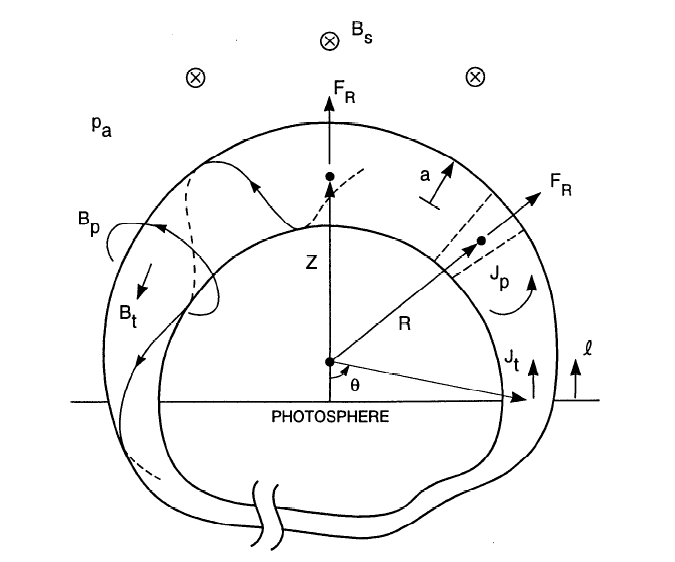
\includegraphics[scale=0.5]{images/chen_model}
\caption{The flux rope model of \citet{chen1989}, used to to study the toroidal instability of a twisted flux system in the corona.}
\label{fig:chen_model}
\end{center}
\end{figure}
The equation of motion of the entire system is given by
\begin{equation}
M\frac{d^2Z}{dt^2} = \frac{I_t}{c^2R}\times\bigg[ \mathrm{ln}\bigg(\frac{8R}{a}\bigg) -1+ \frac{\xi_i}{2} + \frac{\beta_p}{2} -\frac{B^2_t}{B^2_{pa}}  -\frac{2RB_{\perp c}}{aB_{pa}} \bigg] - F_g - F_{drag}
\end{equation}
where $I_t$ is the toroidal current, $R$ is the flux rope major radius, $a$ is the rope minor radius, $\xi_i$ is internal inductance of the flux system, $B_t$ is the toroidal field, $B_{pa}$ is the poloidal field at $a$, $B_{\perp c}$ is the perpendicular component of the ambient coronal field, $F_g$ is the force due to gravity, $F_{drag}$ is the drag force, $M$ is the mass per unit length of the rope, and $Z$ is the rope axis height above the photosphere. The equation of motion shows that an increase in the toroidal current (or poloidal flux) contributes positively to the acceleration. The terms in the square brackets are each unitless and take into account the rope geometry, self-inductance and interplay between poloidal and toroidal flux. The first three terms in the square brackets are what give rise to the hoop-force. If the rope is mass loaded with a prominence, this can contribute to the rope's stability via the gravity term. The drag term only becomes an important contributor to rope dynamics later in the propagation, when the solar wind speed begins to increase i.e., at around 10$R_{\odot}$ reference Sheeley. The eruption is driven by flux-injection, which typically lasts for 4-8 hours, during which time the unstable system loses its equilibrium and begins to rise \citet{krall2001}.

It is significant the fluxrope is already established in the corona before eruption begins i.e., the rope formation is not addressed in the model and it is not a consequence of eruption. Hence magnetic reconnection is not a necessary aspect of the model and the eruption may proceed without employing resistive MHD.


\subsection{Drag Models}\label{sec:23}


\section{Coronal Shocks and Plasma Emission}\label{sec:3}

\subsection{Shock Particle Acceleration}\label{sec:30}

\subsection{Wave-Particle Interaction}\label{sec:31}

Quasi-linear relaxation
\begin{figure}[!t]
\begin{center}
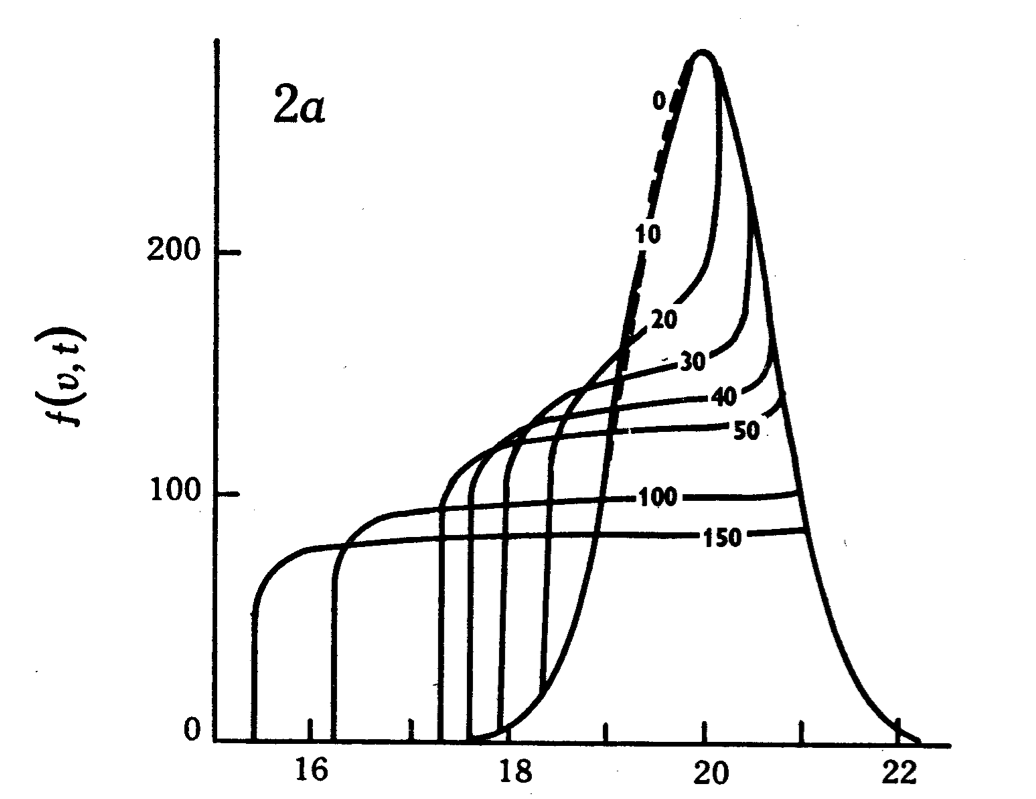
\includegraphics[scale=0.35, trim = 4cm 0cm 0cm 0cm]{images/Grognard1975}
\end{center}
\end{figure}


\subsection{Three-Wave Interaction and Plasma Emission}\label{sec:32}

Once the Langmuir waves are produced from the bump-on-tail instability a number of wave interaction processes occur in order to bring about plasma emission. This involves the interaction of various wave modes in the plasma described by a mathematical formalism called the three-wave interaction. In this process three wave modes in a plasma M, P, and Q are described by their distribution functions in a wave-number space ($k$-space). the distribution functions are given by $N_M(k_M)$, $N_P(k_P)$, $N_Q(k_Q)$, where the $N$ describe the occupation number of wave quanta between $k$ and $k+dk$ in the wave-number space. Waves in P and Q mode may interact to such that wave quanta are removed from the P and Q k-space and added to the M k-space. This is essentially an emission of an energy packet from the P and Q -space to the M k-space. The rate of change of occupation numbers in the three k-spaces are given by
\begin{equation}
\frac{dN_M(\mathbf{k}_M)}{dt} = -\int \frac{d^3\mathbf{k}_P}{(2\pi)^3}\int \frac{d^3\mathbf{k}_Q}{(2\pi)^3}g(\mathbf{k}_M, \mathbf{k}_P, \mathbf{k}_Q)
\end{equation}
\begin{equation}
\frac{dN_P(\mathbf{k}_P)}{dt} = -\int \frac{d^3\mathbf{k}_M}{(2\pi)^3}\int \frac{d^3\mathbf{k}_Q}{(2\pi)^3}g(\mathbf{k}_M, \mathbf{k}_P, \mathbf{k}_Q)
\end{equation}
\begin{equation}
\frac{dN_Q(\mathbf{k}_Q)}{dt} = -\int \frac{d^3\mathbf{k}_M}{(2\pi)^3}\int \frac{d^3\mathbf{k}_P}{(2\pi)^3}g(\mathbf{k}_M, \mathbf{k}_P, \mathbf{k}_Q)
\end{equation}
where $g(\bf{k}_M, \bf{k}_P, \bf{k}_Q)$ is incorporates a transition probability for wave quanta into and out of energy states in the various k-spaces \citep{robinson1994}. The transition probability is given by
\begin{multline}
g(\mathbf{k}_M, \mathbf{k}_P, \mathbf{k}_Q) = u_{MPQ}(\mathbf{k}_M, \mathbf{k}_P, \mathbf{k}_Q)   [N_M(\mathbf{k_M}) N_P(\mathbf{k_P})  - \\ 
N_P(\mathbf{k_P}) N_Q(\mathbf{k_Q})   +N_Q(\mathbf{k_Q}) N_M(\mathbf{k_M})  ]
\end{multline}
where $u_{MPQ}(\bf{k}_M, \bf{k}_P, \bf{k}_Q) $ is the transition probability from states in P and Q  to M, for example \citep{melrose1986}. $u_{MPQ}$ is analogous to transition probabilities given by the Einstein coefficients for transferring energy packets from and atomic state to a photon state (photon emission) i.e., whereas the Einstein coefficients are used in atom-wave (atom-photon) energy exchanges, $u_{MPQ}$ describes wave-wave energy exchanges. The transition probability is given by
\begin{equation}
u_{MPQ}(\mathbf{k}_M, \mathbf{k}_P, \mathbf{k}_Q)  \propto \delta(\omega_M - \omega_P - \omega_Q ) \delta^3(\mathbf{k}_M - \mathbf{k}_P - \mathbf{k}_Q )
\end{equation}
where the $\omega$ are the frequency of the corresponding wave and and $\delta$ are delta functions. Given the presence of delta functions in the transition probability expression, we can see that an exchange of energy quanta amongst the wave modes can only occur when 
\begin{eqnarray}
\omega_M & = & \omega_P + \omega_Q \\
\mathbf{k}_M & = & \mathbf{k}_P + \mathbf{k}_Q
\end{eqnarray}

Hence for an a conversion wave modes in a plasma such as $M \rightarrow P + Q$ (a decay of mode M into P and Q), or it's reverse process $P + Q \rightarrow M $ (a coupling of P and Q to produce M) is described by equations (2.1) to (2.7). 

The production of plasma emission after a bump-on-tail instability has occurred requires a three wave interaction amongst a Langmuir wave $L$, ion acoustic wave $S$, and electromagnetic wave $T$. Fundamental emission during a radio burst occurs via a decay of Langmuir waves into an electromagnetic and ion sound wave
\begin{equation}
L \rightarrow T + S
\end{equation}
while second harmonic first requires the decay $L\rightarrow L^{'} + S$, where $L^{'}$ is a product Langmuir wave propagating in the opposite direction to the first. This is followed by a coalescence of the original and product Langmuir waves
\begin{equation}
L + L^{'}\rightarrow T'
\end{equation}


\begin{itemize}
\item The dispersion relations
\item Source emissivities
\end{itemize}


